\documentclass[10pt,a4paper]{article}
\usepackage[margin = 0.75in]{geometry}
\usepackage{graphicx}
\usepackage{amsmath}
\usepackage{array}
\usepackage{enumitem}
\usepackage{wrapfig}
\usepackage{titlesec}
\usepackage[colorlinks=false]{hyperref}

\titleformat{\section}{\scshape\raggedright}{}{0em}{}
\renewcommand\labelitemi{\raisebox{0.4ex}{\tiny$\bullet$}}
\renewcommand{\labelitemii}{$\cdot$}
\pagenumbering{gobble}

\title{BOX2D PROJECT REPORT}
\begin{document}
\maketitle
\section*{\textbf{Percentage contribution:}}
\textbf{Group name: Tri/ode}\\
\textbf{Rana Prathap(140050068)} : part of code, part of report, part of webpage,
git, presentationslides,(100 percent)\\
\textbf{Sreenivas(140050078)} :part of code, documentation,part of makefile, part of
webpage, git,(100 percent)\\
\textbf{Srinath(140050080)} : part of code, git, profiling, report, part of makefile,(100 percent)\\ 

 

\section*{\textbf{Original project idea:}}

\begin{itemize}[itemsep = -0.75 mm, leftmargin=*]
\item  A simple Rube Goldberg machine consisting of various elements
including conveyor belt, double pulley.It starts with some simulation of various elements and finally a ball
hits the bowling pin .The project was dsigned as shown below
\end{itemize}

\begin{figure}[!htb]
\begin{center}
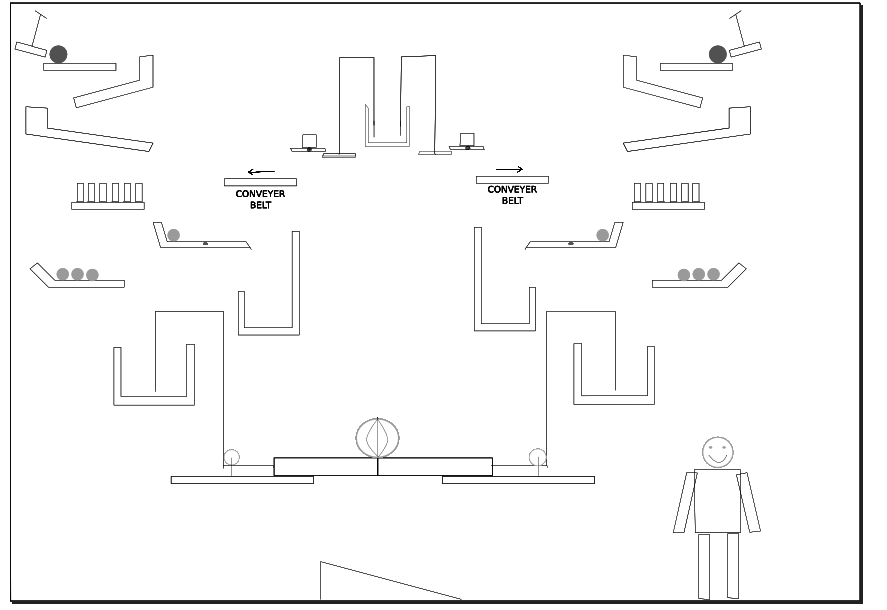
\includegraphics[width=1.0\textwidth]{outline.png}
\end{center}
\caption{Original idea}
\end{figure}

\vspace{-10pt}

\section*{\textbf{What has been implemented:}}
\begin{itemize}[itemsep = -0.75 mm, leftmargin=*]
\item Our final project is almost similar to original idea with very little
deviations, it is shown below.
\end{itemize}

\begin{figure}[!htb]
\begin{center}
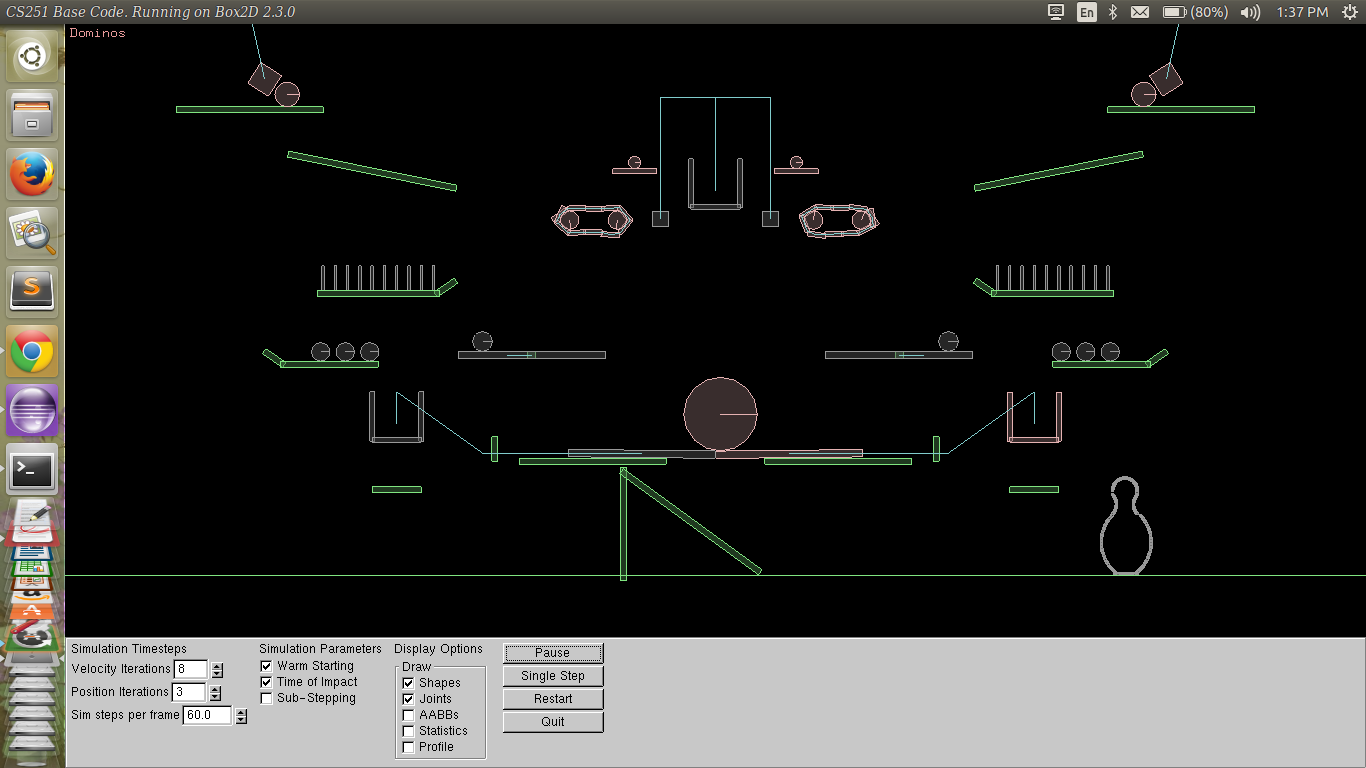
\includegraphics[width=1.0\textwidth]{outlinefinal.png}
\end{center}
\caption{Final Project}
\end{figure}

\vspace{-10pt}
\section*{\textbf{Some thoughts of deviation:}}
\begin{itemize}[itemsep = -0.75 mm, leftmargin=*]
\item We did not deviate much from our original idea. We thought to add
an elastic structure which could throw the large ball towards the bowling pin.
instead of the wedge even it was not part of our original idea, we faced
difficulties there so we sticked to our original idea.
\item We removed the two tray like structures in middle as it didnt look good.We
changed our project name to BOWLING MACHINE and put a bowling pin instead of the
boy.
\end{itemize}
\vspace{-10pt}

\section*{\textbf{Difficulties faced and how we overcame:}}
\begin{itemize}[itemsep = -0.75 mm, leftmargin=*]
 \item We tried implementing the conveyor belt using tangent speed to surfaces
 in contact, we have to change presolve function .\cite{conveyors}
 \item There were many things to be
 changed in other files also and left that idea as we always faced a lot of
 errors. and finally thought to implement via revolute joints.
 \item We tried to make conveyor belt look smooth, so adjusted box widths
 acordingly ,many weired things happened but we finally made it.
 \item We maintained the system perfectly symmetric even then, both the balls
 from conveyor belt did not fall at same pace on the dominos.
 \item Tried to put three pulleys ,but unable to set three anchor points ,so
 changed the function so as to accept three arguments but it led to lot of
 errors so finally restricted to two anchor points
 \item In making the bowling pin we searched for creating arcs in box2d but did
 not find any so implemented it using iteration. 
 \item Thought to include rubber like thread and searched for it ,finally made
 but not used in our project \cite{rubberthread}
 \item Thought to implement mouse drag using mouse joint from box2d manual,
 later found it not that useful.\cite{manual}
\end{itemize}
\vspace{-10pt}

\section*{\textbf{Useful techniqus of lab:}}
 \begin{itemize}[itemsep = -0.75 mm, leftmargin=*]
  \item Git : It was most useful for transfering our files to each other and
  maintain a version control system
  \item diff : We used diff to check the differences in left and right parts as
  simulation is symmetric about vertical axis, we have to maintain the positions
  symmetric
  \item Html : We used all things learnt in lab about html ,css in the project
  webpage, and also adding video to html learnt from one of inlabs
  \item Makefiles : used to make our own makefile of this project
  \item Latex and Beamer : of course used to make this project report and the
  presentation
 \end{itemize}
\vspace{-10pt}

\section*{\textbf{Some stages of our project:}}
 \begin{itemize}[itemsep = -0.75 mm, leftmargin=*]
  \item below shown figures are at some stages of our project
 \end{itemize}
 
 \begin{figure}[!htb]
 \begin{centering}
 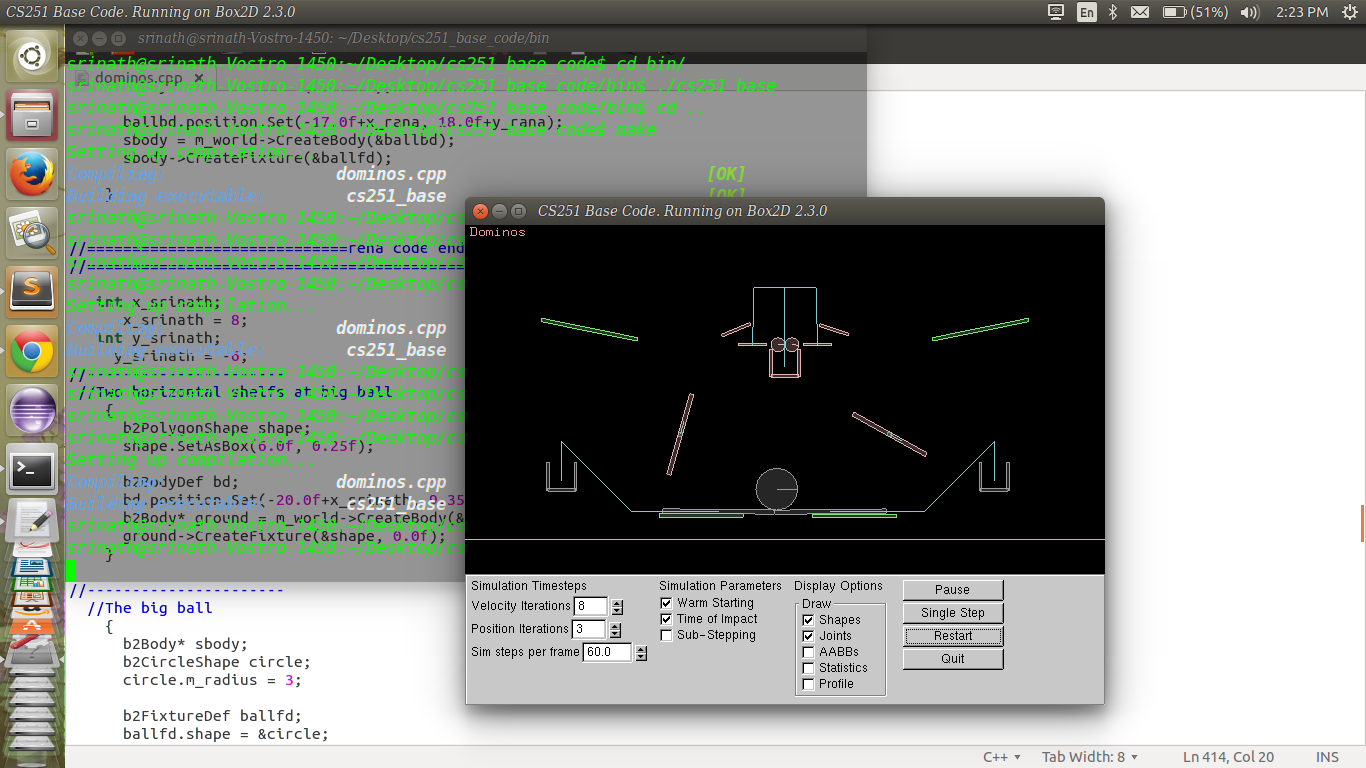
\includegraphics[width=0.5\textwidth]{bareinitial.png}
 \end{centering}
 \caption{Just started}
 \end{figure}
 \vspace{-10pt}
  
  \begin{itemize}[itemsep = -0.75 mm, leftmargin=*]
  \item Later suffered with conveyor belt and the dominos and it looks as..
 \end{itemize}

 \begin{figure}[!htb]
 \begin{centering}
 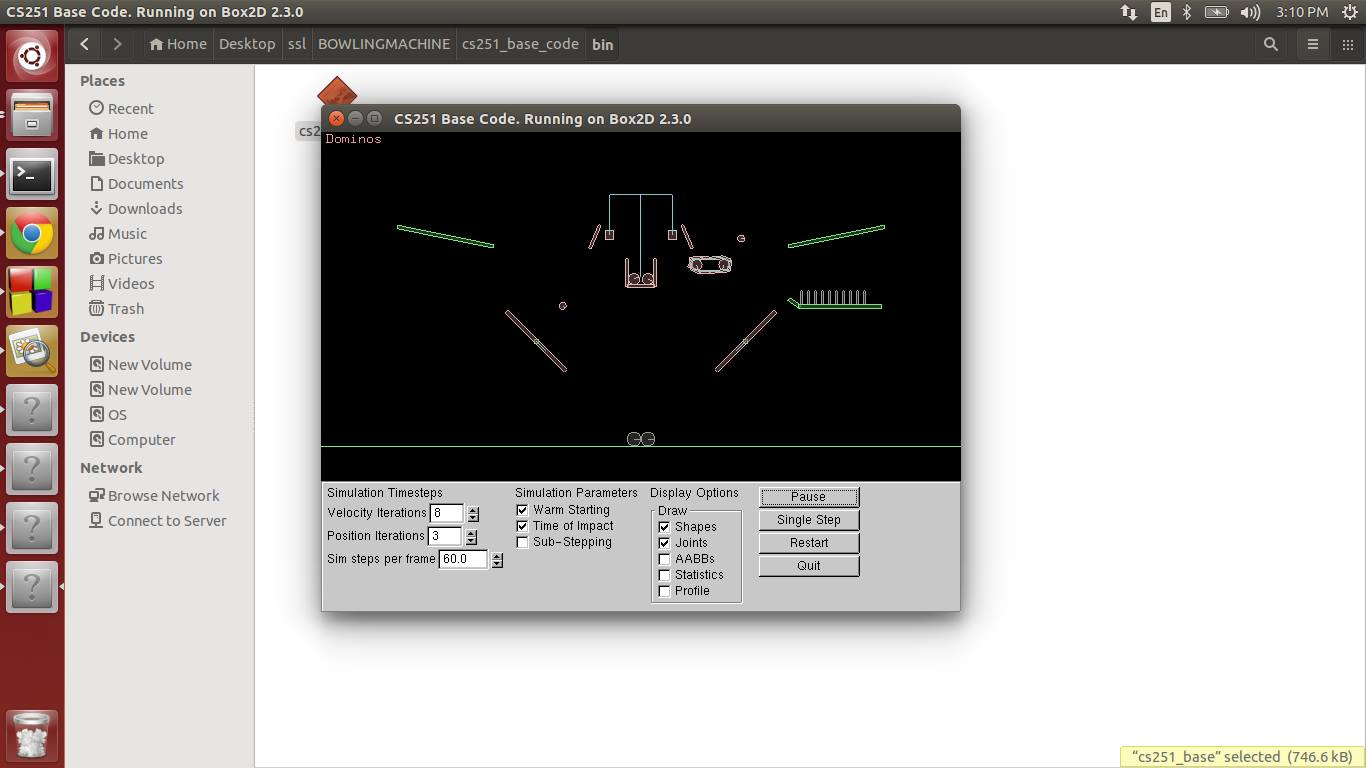
\includegraphics[width=0.5\textwidth]{middle.jpg}
 \end{centering}
 \caption{Fixing conveyor belt}
 \end{figure}
 \vspace{-10pt}
 
  \begin{itemize}[itemsep = -0.75 mm, leftmargin=*]
  \item Finally united the objects and got our prefinal project..
 \end{itemize}

 \begin{figure}[!htb]
 \begin{centering}
 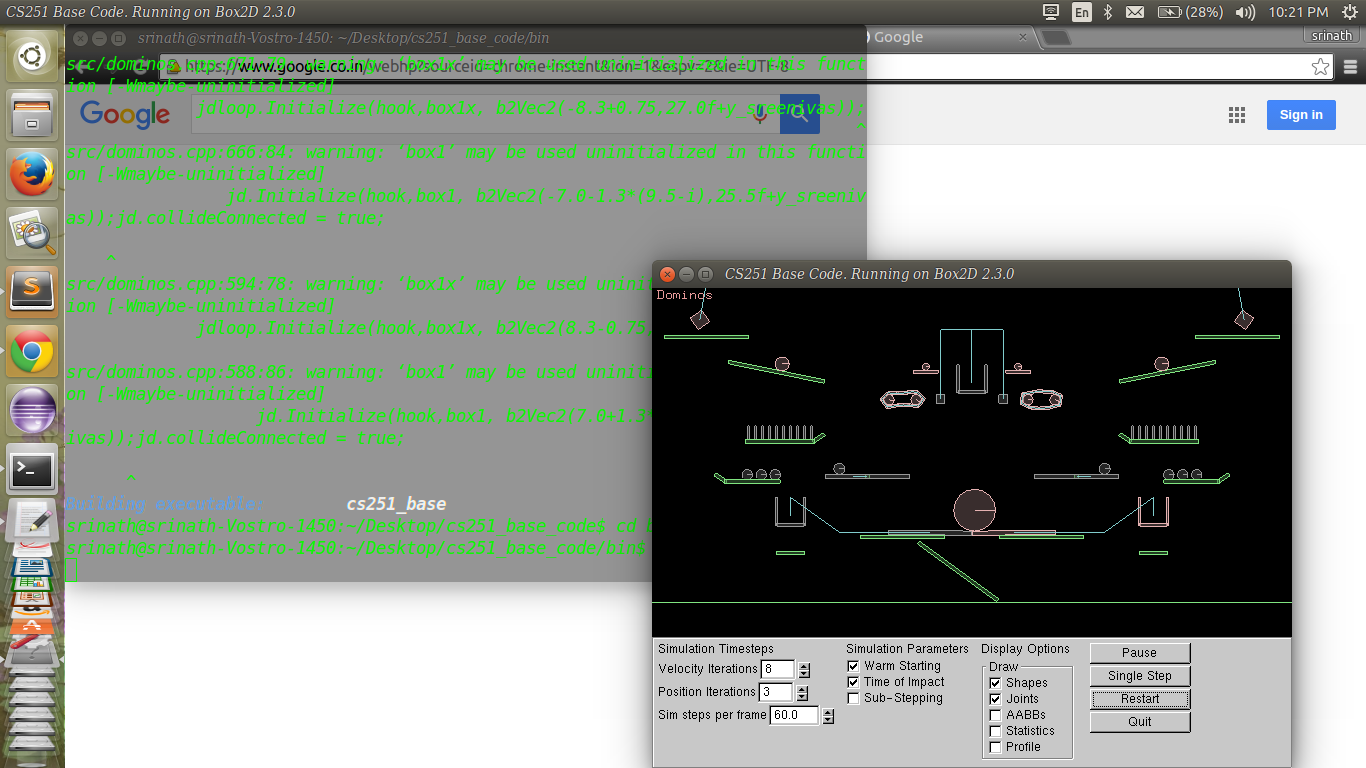
\includegraphics[width=0.5\textwidth]{prefinal.png}
 \end{centering}
 \caption{almost done}
 \end{figure}
 \vspace{-10pt}
 
 \section*{\textbf{Profiling Data:}}
   \begin{itemize}
   \item The call graph our final project code in is shown here
    \end{itemize}  
 \begin{figure}[!htb]
 \begin{centering}
 
\includegraphics[width=5.0\textwidth]{final.png}
 \end{centering}
 \caption{Final call graph}
 \end{figure}
 \vspace{-10pt}
      
   \begin{itemize}
    \item The call graph for release mode of final project is also shown
   \end{itemize}

 \begin{figure}[!htb]
 \begin{centering}
 
\includegraphics[width=5.0\textwidth]{final_release.png}
 \end{centering}
 \caption{Final call graph release mode}
 \end{figure}
 \vspace{-10pt}  

   \begin{itemize}
   \item The call graph of original cs251 base code is below
   \item The top functions in original base code are
   b2world::DrawShape(b2Fixture, b2Transform, b2color const)about 13 percent ,
   DrawSolidCircle(b2vect2 const,float, b2vect2 const, b2color const)about 9.7
   percent
   \item The top functions in  our code are Operator(b2vect, b2vect2 const )
   about 8 percent, b2vect2::b2vect2(float,float) about 6.4 percent
   \item The differences are probably because of increased fixtures(bars) and
   pulleys in our code than that of original base code
   \end{itemize}
   
 \begin{figure}[!htb]
 \begin{centering}
 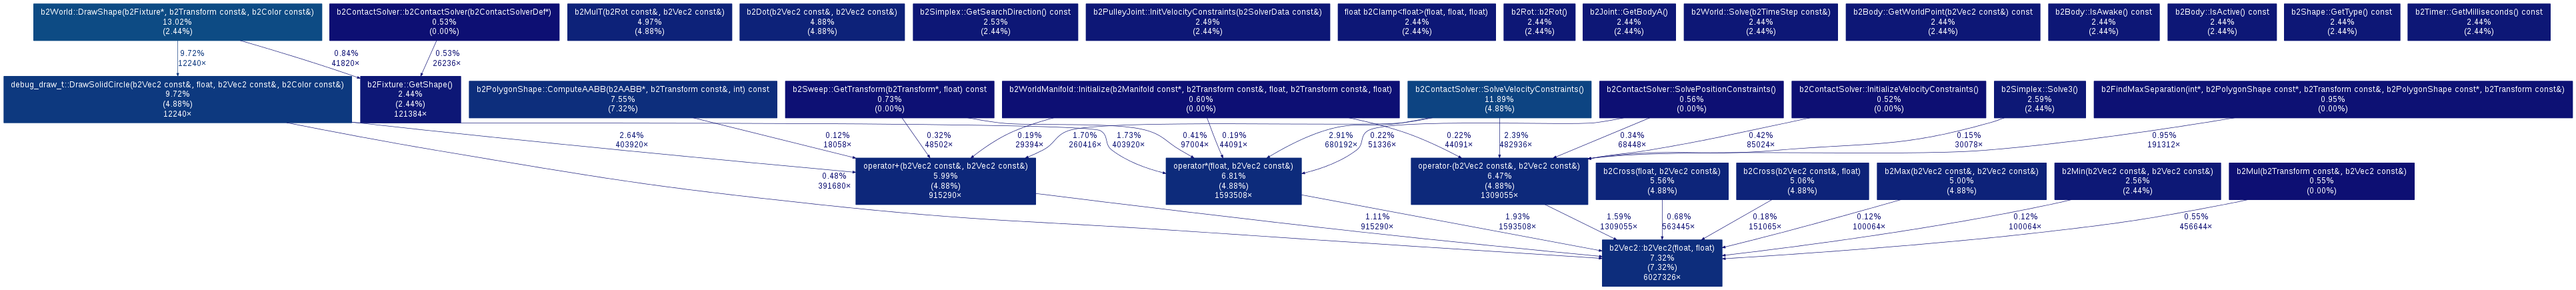
\includegraphics[width=1.0\textwidth]{final251base.png}
 \end{centering}
 \caption{Final 251base call graph}
 \end{figure}
 \vspace{-10pt}
   
\section*{\textbf{Sources used:}}
 \begin{itemize}[itemsep = -0.75 mm, leftmargin=*]
  \item Some of the tutorials from this site \cite{boxtut}
  \item Many other sourses are mentioned in the references list
 \end{itemize}
\section*{\textbf{Honour code:}}
We pledge on my honour that we have not given or received any unauthorized
assistance on this    assignment or any previous task.
  \bibliographystyle{plain}
  \bibliography{bibfile}

\end{document}
